\section{Details of the Optimization Argument}
\label{app:proof}
\subsection{Orthogonal projection and retained energy}
Let $x_i=\operatorname{vec}(\mathcal X_i)$ and
$P=U_K\otimes\cdots\otimes U_1$. The Kronecker product identities give
$P^\top P=(U_K^\top U_K)\otimes\cdots\otimes(U_1^\top U_1)=I$.
Thus $Q=PP^\top$ is symmetric and idempotent, so
\begin{equation}
\|x_i-Qx_i\|_2^2
=x_i^\top(I-Q)^2x_i
=\|x_i\|_2^2-x_i^\top Qx_i
=\|x_i\|_2^2-\|P^\top x_i\|_2^2.
\end{equation}
Since $P^\top x_i=\operatorname{vec}(\mathcal Y_i)$, summation yields the energy
identity in Section~\ref{sec:methods}. This identity holds without centering;
centering is needed for the usual variance interpretation.

\subsection{Why the eigenvector update is optimal}
For three-mode tensors, fixing $U_2,U_3$ gives
$B_i=(\mathcal X_i\times_2U_2^\top\times_3U_3^\top)_{(1)}$.
Both $B_i$ and $C_1=\sum_iB_iB_i^\top$ stay fixed while optimizing $U_1$.
Because unfolding preserves the Frobenius norm,
$\sum_i\|U_1^\top B_i\|_F^2=\operatorname{tr}(U_1^\top C_1U_1)$.
The same argument applies to every mode.

Write $C_k=V\Lambda V^\top$, with orthonormal eigenvectors $v_j$ and descending
eigenvalues $\lambda_j$. Any feasible $U$ satisfies
\begin{equation}
\operatorname{tr}(U^\top C_kU)=\sum_j\lambda_jw_j,
\quad w_j=\|v_j^\top U\|_2^2\in[0,1],
\quad\sum_jw_j=r_k.
\end{equation}
The bounds follow because $UU^\top$ is a rank-$r_k$ orthogonal projector.
The weighted sum is at most $\sum_{j=1}^{r_k}\lambda_j$, attained by
$U=[v_1,\ldots,v_{r_k}]$. Since the old basis is feasible, this proves
Equation~\eqref{eq:nonincrease}, expanding Theorem~1 of \citet{xu2008csa}.
Successive exact updates satisfy
$E^{(t,0)}\geq E^{(t,1)}\geq\cdots\geq E^{(t,K)}=E^{(t+1,0)}\geq0$.
Ranks, data, and preprocessing remain fixed. Equality and nonunique bases can
occur, especially with repeated eigenvalues; objective convergence does not
prove convergence of the bases or a strict local minimum. Numerical checks
must allow floating-point tolerance.

\section{Reproduction Protocols and Supplementary Evidence}
\label{app:protocol}
\subsection{Inputs, splits, and implementation choices}
ORL contains 400 images from 40 identities \citep{orlData}. Recognition uses
aligned/equalized $56\times46$ grayscale images or $28\times23\times40$ Gabor
magnitudes. The current comparison uses seeds 20--29, shared inputs and
Euclidean 1-NN, with unit-length LDA columns. CSA runs at most three sweeps;
CSA24 uses HOSVD initialization, while grayscale/direct CSA390 use rectangular
identity bases. The $\pi$-context Gabor input filters an expanded aligned image
before extracting the central response. It is a declared extension, not an
author-confirmed preprocessing choice. All current ORL inputs retain previous
probe-informed development; the final fixed batch performs no new search but
is not an independent blind test.

For the metric comparison, the gallery feature mean is subtracted from both
gallery and probe embeddings before scoring. This common translation leaves
Euclidean distances unchanged but defines the centered-cosine rule. The fitted
CSA/PCA/LDA maps remain fixed; this scoring step is distinct from centering
the training inputs when fitting PCA.

MNIST uses the first 500 images of each digit in the official test set,
5,000 images total \citep{lecun1998mnist}, with $28\times28\times40$ Gabor features.
Each split selects 30 or 40 training examples per class, leaving 470 or 460
probes. The original paper describes the ``first half'' of the test set and
also 500 images per class; our balanced selection is explicit, but the authors'
exact indices are unavailable. The recognition dimensions are listed in
Table~\ref{tab:configurations}; the distance is cosine.

We use original grayscale FERET \citep{phillips2000feret}, with 1,195 Fa/Fb
identity pairs as in \citet[Sec.~IV-A]{xu2008csa}, aligned/equalized to $41\times27$.
For $q=50,100,200$, the first $q$ paired identities provide training Fa+Fb;
remaining Fa images form the gallery and Fb images the probes. The table uses
fixed cosine controls, not validation-selected winners.
Identity ordering and precise alignment conventions are not confirmed identical
to the paper. Recognition PCA is centered and CSA uncentered in all three datasets.

The group implements the learning and evaluation algorithms; scientific
libraries, BLAS/LAPACK, image utilities, and pretrained detectors are reused
components. The repository documents dependencies, data acquisition, model
settings, source attribution, and verification. Raw datasets and feature/model
caches are not distributed; regenerating full checks requires the data and
documented preparation stages. This report audits saved records and does not
claim a fresh end-to-end rerun.

\subsection{Exact recognition configurations}
\begin{table}[!ht]
\centering
\small
\setlength{\tabcolsep}{4pt}
\caption{Recorded group configurations for the eight comparisons in
Table~\ref{tab:recognition}. An arrow gives the output dimension after LDA;
no arrow means direct 1-NN. The CSA tuple lists mode ranks, not only their
product. $G$ is training images per digit and $q$ is training identities.
These recognition runs use centered PCA and uncentered CSA.}
\label{tab:configurations}
\begin{tabular}{@{}llllr@{}}
\toprule
Setting & PCA $\to$ LDA & CSA ranks $\to$ LDA & Distance & Splits\\
\midrule
ORL gray & $30\to18$ & $11\times2\to16$ & Euclidean & 10\\
ORL Gabor, direct & $76$ & $15\times1\times26$ & Euclidean & 10\\
ORL Gabor + LDA & $33\to25$ & $4\times2\times3\to23$ & Euclidean & 10\\
MNIST, $G=30$ & $60$ & $5\times9\times18$ & Cosine & 3\\
MNIST, $G=40$ & $50$ & $15\times5\times13$ & Cosine & 3\\
FERET, $q=50$ & $45\to25$ & $10\times4\to35$ & Cosine & 1\\
FERET, $q=100$ & $95\to40$ & $11\times5\to44$ & Cosine & 1\\
FERET, $q=200$ & $112\to69$ & $13\times7\to62$ & Cosine & 1\\
\bottomrule
\end{tabular}
\end{table}
\FloatBarrier
For the matched-dimension control in Figure~\ref{fig:metric}, PCA changes to
$24\to23$, while CSA remains $4\times2\times3\to23$.
Changing the distance does not refit these models. The table records the
implemented rank allocation; unavailable author code and input settings
prevent a claim of completely author-identical pipelines.

\subsection{Controlled extensions and traceable records}
\label{app:controls}
The 20-split $\sigma=\pi$ crop/context comparison uses centered cosine and fixed
$24\to23$ dimensions. Filtering beyond the crop changes the effective field of
view, so its benefit cannot be attributed solely to the learned representation.
With five probes held fixed per ORL identity, increasing the gallery from two
to three to five gives CSA+LDA 81.30\%, 88.10\%, and 94.50\%; both the fitting
data and reference coverage change.
Our supervised DATER extension \citep{yan2005dater} reaches
$67.11\pm3.59$\% after LDA versus matched CSA's $80.13\pm3.49$\% in the crop-only
control. However, 19 of 20 DATER runs hit the 20-iteration cap, so this is a
negative result for the tested implementation/configuration, not evidence that
supervised tensor methods generally fail.

{\raggedright
The main table is traceable to
\path{results/orl_euclidean_20261104/comparison.csv} and the MNIST/FERET records in
\path{results/orl_protocol_audit/shared_comparison.csv}.
Metric comparisons use \path{results/orl_euclidean_20261104/paired_comparisons.csv};
input controls and weight counts use \path{results/orl_controlled/summary.csv}
and \path{results/orl_controlled/cost_benchmark.csv}.
The gallery-size and DATER sources are \path{results/orl_sample_size/summary.json}
and \path{results/orl_dater/summary.csv}. Qualitative reconstruction and
convergence are recorded in \path{results/available_reproduction_v2/orl_reconstruction.csv}
and \path{results/available_reproduction_v2/orl_convergence.json}.
These are group results; all paper values in Table~\ref{tab:recognition}
are separately attributed to \citet{xu2008csa}.\par}

\clearpage
\section{Recorded Reconstruction and Convergence Diagnostics}
\label{app:reconstruction}
\subsection{Diagnostic setup and comparison budget}
Figure~\ref{fig:reconstruction} uses our saved historical ORL reconstruction
batch: one image per identity (\path{s*/1.pgm}), $N=40$, with full-resolution
$56\times46\times40$ Gabor tensors, $D=103{,}040$ values per object.
Both PCA and CSA are uncentered, and error is evaluated on those same fitting
images. These inputs use historical Haar-based eye alignment with 16 approximate
visual corrections and $\sigma=2\pi$ reflected-boundary filtering. They differ from
the current YuNet/context recognition inputs. Thus the figure illustrates
compression of fitted objects, not unseen-image generalization or the current
recognition protocol.

For stored scalar count $S$, the recorded definitions are
\begin{equation}
\begin{aligned}
\mathrm{CR}&=\frac{ND}{S},&
\mathrm{RMSE}&=\sqrt{\frac{\mathrm{SSE}}{N}},\\
S_{\mathrm{PCA}}&=d(N+D),&
S_{\mathrm{CSA}}&=Nr^3+(56+46+40)r.
\end{aligned}
\end{equation}
The CSA grid uses equal mode ranks $r=1,\ldots,40$; PCA uses $d=1,\ldots,40$.
Each reconstruction CSA fit allows up to ten sweeps with the usual early
stopping rule enabled.
Storage includes cores and bases, with no mean vector for these uncentered
models. RMSE is per object, not per scalar/pixel. The CSV field
\texttt{paper\_rmse} names this definition; its values are our measurements.
The discrete compression grids differ. As a concrete comparison without
interpolation, PCA with $d=2$ stores 206,160 scalars and has RMSE 3458.78;
CSA with $r=17$ stores fewer scalars (198,934) and has RMSE 1624.32.
This supports an advantage at that storage cap, not superiority at equal
coefficient count or across all budgets.

\subsection{Observed convergence and its limits}
The diagnostic uses a $10\times10\times10$ core and rectangular-identity
initialization. Early stopping is disabled to record ten sweeps; recognition
still uses at most three. SSE falls from $2.570566\times10^9$ at initialization
to $2.039869\times10^8$ after one sweep and $2.033656\times10^8$ after three.
Similarity is the average absolute inner product of corresponding old/new
basis columns. All three recorded similarities exceed $0.9999999$ at sweep
three. Later SSE substep increases are at most approximately $3.34\times10^{-6}$,
about $1.64\times10^{-14}$ relative to the loss, consistent with floating-point
effects rather than a strict numerical decrease at every step.
This is an observed trajectory, not proof of global optimality or a universal
three-sweep guarantee.

\begin{figure}[!ht]
\centering
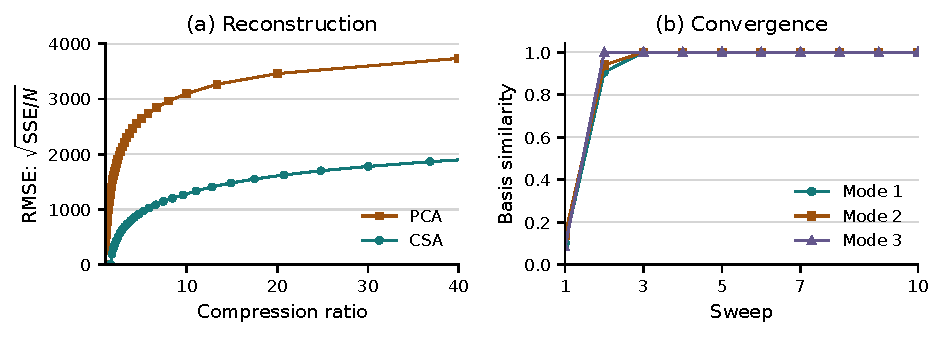
\includegraphics[width=\linewidth]{figures/reconstruction_convergence.pdf}
\caption{Our recorded reconstruction and convergence diagnostics on 40 ORL
fitting images. Left: compression ratio includes basis storage; markers show
recorded settings and connecting lines guide the eye. The displayed range is
restricted to CR $1$--$40$, not the entire CSA grid. Right: successive-basis
similarity for the $10\times10\times10$ diagnostic with early stopping disabled.
These are group records, not digitized paper curves; absolute feature scaling
is not established as author-identical. Sources: the reconstruction and
convergence records listed in Appendix~\ref{app:controls}.}
\label{fig:reconstruction}
\end{figure}
\FloatBarrier
